% The two figures belonging to §4. Held in their own file so that main.tex and review_s4.tex
% share one copy and the export cannot drift from the manuscript.
\begin{figure}[t]
  \centering
  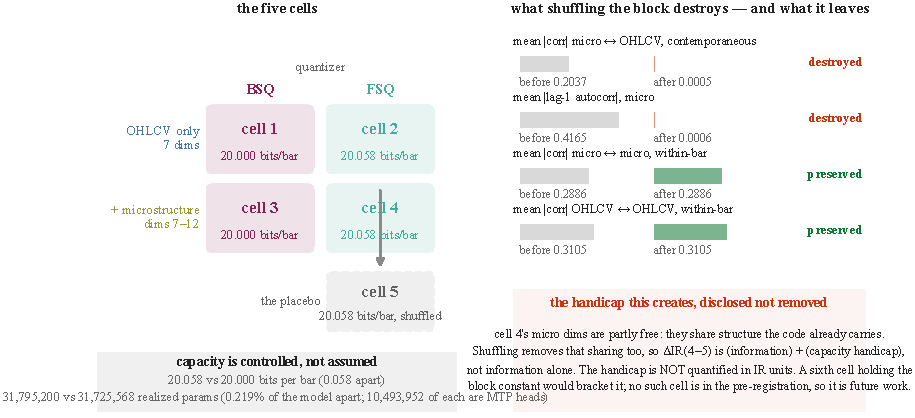
\includegraphics[width=\textwidth]{figures/fig5_design.pdf}
  \caption{\textbf{The five cells, at matched capacity, and the exact reach of the placebo.}
  \emph{Left:} a $2\times2$ over quantizer and input arm, plus a fifth cell that is cell 4 with the
  microstructure block shuffled. Capacity is controlled rather than assumed: the two quantizer arms
  differ by $0.058$ bits per bar and by $0.327\%$ of backbone parameters, so a difference between
  them cannot be attributed to one arm simply having more room. \emph{Right:} what the shuffle
  actually does, measured. It destroys the two things it was built to destroy --- microstructure's
  contemporaneous link to price ($0.2037 \rightarrow 0.0005$) and its own lag-1 autocorrelation
  ($0.4165 \rightarrow 0.0006$) --- and leaves the within-block and within-OHLCV correlations
  exactly as they were. The consequence is stated rather than hidden: because cell 4's
  microstructure dimensions are partly amortized against structure the code already carries,
  shuffling removes that sharing too, so $\Delta$IR(4$-$5) is (information) $+$ (capacity
  handicap). The handicap is not quantified in
  information-ratio units. A sixth cell holding the block constant would bracket it, but no such
  cell appears anywhere in the pre-registration, so it is future work rather than a committed
  contingency, and \cref{sec:limitations} carries the handicap as an open disclosure.}
  \label{fig:design}
\end{figure}
\clearpage
\begin{figure}[t]
  \centering
  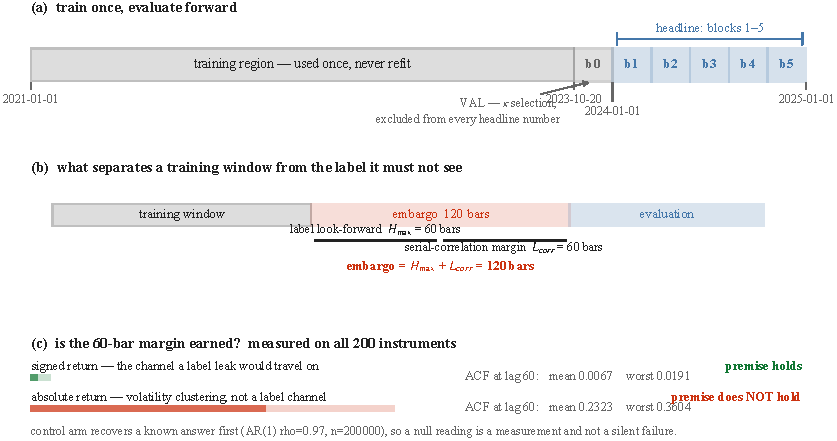
\includegraphics[width=\textwidth]{figures/fig6_validation.pdf}
  \caption{\textbf{Train once, evaluate forward, and pay for the separation.} \textbf{(a)} The training
  region ends at one boundary and is never refit. The forward region is cut into six blocks; block
  0 is spent selecting the execution filter and is excluded from every headline number, so the
  headline is scored on five blocks the selection never saw. \textbf{(b)} Between a training window
  and any label that could contaminate it sit a $60$-bar label look-forward and a $60$-bar
  serial-correlation margin, giving a $120$-bar embargo. \textbf{(c)} The premise behind that
  margin is measured on all $200$ instruments rather than assumed, and a control arm recovers a
  known AR(1) answer first, so a null reading is a measurement and not a silent failure. It holds
  for signed returns --- the channel a label leak would travel on --- at ACF $0.0067$ mean and
  $0.0191$ worst-symbol at lag $60$. It does \emph{not} hold for absolute returns
  ($0.2323$ mean, $0.3604$ worst), which is volatility clustering rather than a label channel;
  \cref{sec:limitations} carries that caveat.}
  \label{fig:validation}
\end{figure}
